
\documentclass[border=10pt, 12pt]{standalone}
\usepackage[svgnames]{xcolor}
\usepackage{amsmath}
\usepackage{pgfplots}
\pgfplotsset{compat=newest}
\usepackage[sfdefault]{FiraSans}
\usepackage{FiraMono}
\renewcommand*\familydefault{\sfdefault}
\begin{document}
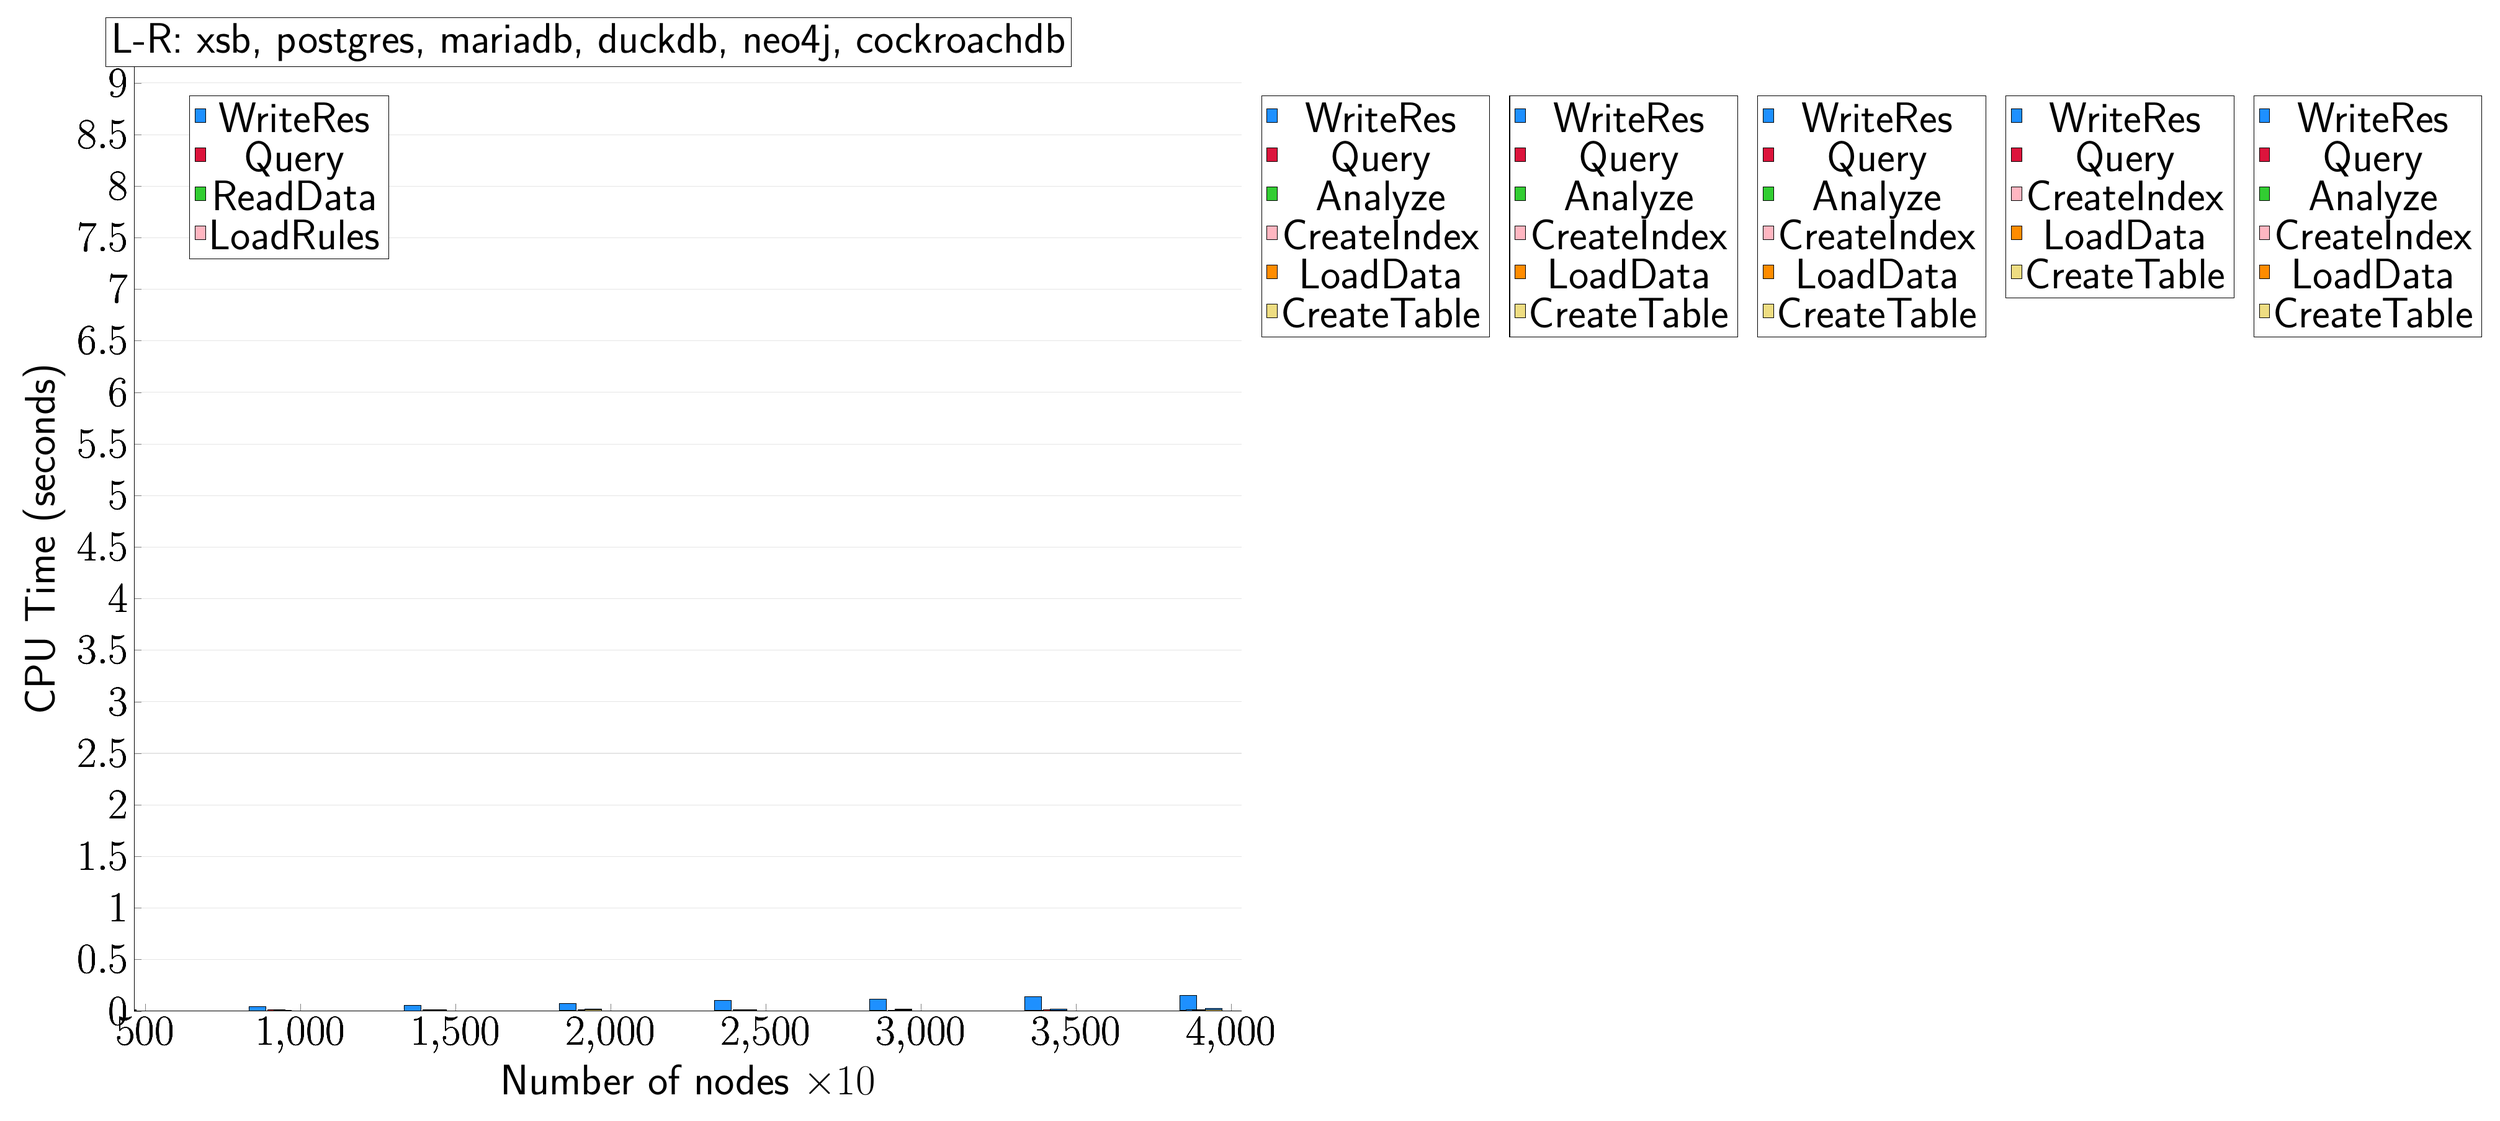
\begin{tikzpicture}
                        \begin{axis}[bar shift=-25pt, 
   ybar stacked,
   width=2\textwidth,
   bar width=0.35cm,
   ymajorgrids, tick align=inside,
   major grid style={draw=gray!20},
   xtick=data,
   ymin=0, ymax=9.153333336114883,
   axis x line*=bottom,
   axis y line*=left,
   enlarge x limits=0.01,
   legend style={
       at={(0.23, 0.97)},
       anchor=north east,
       legend columns=1,
       font=\Huge,
   },
   ylabel={CPU Time (seconds)},
   xlabel={Number of nodes $\times 10$},
   label style={font=\Huge},
   tick label style={font=\Huge},
]
\addlegendimage{fill=DodgerBlue, draw=black, line width=0.2pt}
\addlegendentry{WriteRes}
\addlegendimage{fill=Crimson, draw=black, line width=0.2pt}
\addlegendentry{Query}
\addlegendimage{fill=LimeGreen, draw=black, line width=0.2pt}
\addlegendentry{ReadData}
\addlegendimage{fill=LightPink, draw=black, line width=0.2pt}
\addlegendentry{LoadRules}
\addplot +[fill=LightPink, draw=black, line width=0.2pt] coordinates {
(500, 0.0034230000000000003)
(1000, 0.0033439999999999998)
(1500, 0.0025943333333333335)
(2000, 0.003172333333333333)
(2500, 0.0027816666666666667)
(3000, 0.0029416666666666666)
(3500, 0.00364566666666667)
(4000, 0.0035303333333333332)
};
\addplot +[fill=LimeGreen, draw=black, line width=0.2pt] coordinates {
(500, 0.0012956666666666674)
(1000, 0.0020723333333333336)
(1500, 0.001815)
(2000, 0.0030310000000000003)
(2500, 0.003395666666666663)
(3000, 0.003058333333333333)
(3500, 0.004817666666666667)
(4000, 0.005053666666666667)
};
\addplot +[fill=Crimson, draw=black, line width=0.2pt] coordinates {
(500, 0.0001193333333333323)
(1000, 0.00021800000000000066)
(1500, 0.000213999999999999)
(2000, 0.0004353333333333293)
(2500, 0.00047300000000000234)
(3000, 0.000616666666666666)
(3500, 0.000714666666666669)
(4000, 0.0007363333333333342)
};
\addplot +[fill=DodgerBlue, draw=black, line width=0.2pt] coordinates {
(500, 0.018995)
(1000, 0.037186)
(1500, 0.05008933333333334)
(2000, 0.06862366666666667)
(2500, 0.09641466666666666)
(3000, 0.11093966666666666)
(3500, 0.1302576666666667)
(4000, 0.14466066666666666)
};
\end{axis}

\begin{axis}[bar shift=-21.3pt, 
   ybar stacked,
   width=2\textwidth,
   bar width=0.35cm,
   ymajorgrids, tick align=inside,
   major grid style={draw=none},
   xtick=data,
   ymin=0, ymax=9.153333336114883,
   axis x line*=none,
   axis y line*=none,
   enlarge x limits=0.01,
   legend style={
       at={(1.224, 0.97)},
       anchor=north east,
       legend columns=1,
       font=\Huge,
   },
   label style={font=\Huge},
   tick label style={font=\Huge},
]
\addlegendimage{fill=DodgerBlue, draw=black, line width=0.2pt}
\addlegendentry{WriteRes}
\addlegendimage{fill=Crimson, draw=black, line width=0.2pt}
\addlegendentry{Query}
\addlegendimage{fill=LimeGreen, draw=black, line width=0.2pt}
\addlegendentry{Analyze}
\addlegendimage{fill=LightPink, draw=black, line width=0.2pt}
\addlegendentry{CreateIndex}
\addlegendimage{fill=DarkOrange, draw=black, line width=0.2pt}
\addlegendentry{LoadData}
\addlegendimage{fill=LightGoldenrod, draw=black, line width=0.2pt}
\addlegendentry{CreateTable}
\addplot +[fill=LightGoldenrod, draw=black, line width=0.2pt] coordinates {
(500, 0.0)
(1000, 0.0)
(1500, 0.0)
(2000, 0.0)
(2500, 0.0)
(3000, 0.0)
(3500, 0.0)
(4000, 0.0)
};
\addplot +[fill=DarkOrange, draw=black, line width=0.2pt] coordinates {
(500, 0.0)
(1000, 0.0)
(1500, 0.0)
(2000, 0.0)
(2500, 0.0)
(3000, 0.0)
(3500, 0.0)
(4000, 0.0)
};
\addplot +[fill=LightPink, draw=black, line width=0.2pt] coordinates {
(500, 0.0)
(1000, 0.0)
(1500, 0.0)
(2000, 0.0)
(2500, 0.0)
(3000, 0.0)
(3500, 0.0)
(4000, 0.0)
};
\addplot +[fill=LimeGreen, draw=black, line width=0.2pt] coordinates {
(500, 0.0)
(1000, 0.0)
(1500, 0.0)
(2000, 0.0)
(2500, 0.0)
(3000, 0.0)
(3500, 0.0)
(4000, 0.0)
};
\addplot +[fill=Crimson, draw=black, line width=0.2pt] coordinates {
(500, 0.0)
(1000, 0.0)
(1500, 0.0)
(2000, 0.0)
(2500, 0.0)
(3000, 0.0)
(3500, 0.0)
(4000, 0.0)
};
\addplot +[fill=DodgerBlue, draw=black, line width=0.2pt] coordinates {
(500, 0.0)
(1000, 0.0)
(1500, 0.0)
(2000, 0.0)
(2500, 0.0)
(3000, 0.0)
(3500, 0.0066666666666666706)
(4000, 0.013333333333333343)
};
\end{axis}

\begin{axis}[bar shift=-17.6pt, 
   ybar stacked,
   width=2\textwidth,
   bar width=0.35cm,
   ymajorgrids, tick align=inside,
   major grid style={draw=none},
   xtick=data,
   ymin=0, ymax=9.153333336114883,
   axis x line*=none,
   axis y line*=none,
   enlarge x limits=0.01,
   legend style={
       at={(1.448, 0.97)},
       anchor=north east,
       legend columns=1,
       font=\Huge,
   },
   label style={font=\Huge},
   tick label style={font=\Huge},
]
\addlegendimage{fill=DodgerBlue, draw=black, line width=0.2pt}
\addlegendentry{WriteRes}
\addlegendimage{fill=Crimson, draw=black, line width=0.2pt}
\addlegendentry{Query}
\addlegendimage{fill=LimeGreen, draw=black, line width=0.2pt}
\addlegendentry{Analyze}
\addlegendimage{fill=LightPink, draw=black, line width=0.2pt}
\addlegendentry{CreateIndex}
\addlegendimage{fill=DarkOrange, draw=black, line width=0.2pt}
\addlegendentry{LoadData}
\addlegendimage{fill=LightGoldenrod, draw=black, line width=0.2pt}
\addlegendentry{CreateTable}
\addplot +[fill=LightGoldenrod, draw=black, line width=0.2pt] coordinates {
(500, 0.0)
(1000, 0.0)
(1500, 0.0)
(2000, 0.0)
(2500, 0.0)
(3000, 0.0)
(3500, 0.0)
(4000, 0.0)
};
\addplot +[fill=DarkOrange, draw=black, line width=0.2pt] coordinates {
(500, 0.0)
(1000, 0.0)
(1500, 0.0)
(2000, 0.0)
(2500, 0.0)
(3000, 0.0)
(3500, 0.0)
(4000, 0.0)
};
\addplot +[fill=LightPink, draw=black, line width=0.2pt] coordinates {
(500, 0.0)
(1000, 0.0)
(1500, 0.0)
(2000, 0.003333333333333336)
(2500, 0.0)
(3000, 0.0)
(3500, 0.0)
(4000, 0.0)
};
\addplot +[fill=LimeGreen, draw=black, line width=0.2pt] coordinates {
(500, 0.0)
(1000, 0.0)
(1500, 0.0)
(2000, 0.0)
(2500, 0.0)
(3000, 0.0)
(3500, 0.0)
(4000, 0.0)
};
\addplot +[fill=Crimson, draw=black, line width=0.2pt] coordinates {
(500, 0.0)
(1000, 0.0)
(1500, 0.0)
(2000, 0.0)
(2500, 0.0)
(3000, 0.0)
(3500, 0.0)
(4000, 0.0)
};
\addplot +[fill=DodgerBlue, draw=black, line width=0.2pt] coordinates {
(500, 0.0)
(1000, 0.0)
(1500, 0.0)
(2000, 0.0)
(2500, 0.0)
(3000, 0.0)
(3500, 0.0)
(4000, 0.0066666666666666706)
};
\end{axis}

\begin{axis}[bar shift=-13.899999999999999pt, 
   ybar stacked,
   width=2\textwidth,
   bar width=0.35cm,
   ymajorgrids, tick align=inside,
   major grid style={draw=none},
   xtick=data,
   ymin=0, ymax=9.153333336114883,
   axis x line*=none,
   axis y line*=none,
   enlarge x limits=0.01,
   legend style={
       at={(1.6720000000000002, 0.97)},
       anchor=north east,
       legend columns=1,
       font=\Huge,
   },
   label style={font=\Huge},
   tick label style={font=\Huge},
]
\addlegendimage{fill=DodgerBlue, draw=black, line width=0.2pt}
\addlegendentry{WriteRes}
\addlegendimage{fill=Crimson, draw=black, line width=0.2pt}
\addlegendentry{Query}
\addlegendimage{fill=LimeGreen, draw=black, line width=0.2pt}
\addlegendentry{Analyze}
\addlegendimage{fill=LightPink, draw=black, line width=0.2pt}
\addlegendentry{CreateIndex}
\addlegendimage{fill=DarkOrange, draw=black, line width=0.2pt}
\addlegendentry{LoadData}
\addlegendimage{fill=LightGoldenrod, draw=black, line width=0.2pt}
\addlegendentry{CreateTable}
\addplot +[fill=LightGoldenrod, draw=black, line width=0.2pt] coordinates {
(500, 0.0)
(1000, 0.0)
(1500, 0.0)
(2000, 0.003333333333333336)
(2500, 0.006666666666666669)
(3000, 0.0)
(3500, 0.0)
(4000, 0.0)
};
\addplot +[fill=DarkOrange, draw=black, line width=0.2pt] coordinates {
(500, 0.0)
(1000, 0.003333333333333336)
(1500, 0.003333333333333336)
(2000, 0.0)
(2500, 0.0)
(3000, 0.003333333333333336)
(3500, 0.0)
(4000, 0.0)
};
\addplot +[fill=LightPink, draw=black, line width=0.2pt] coordinates {
(500, 0.003333333333333336)
(1000, 0.0)
(1500, 0.003333333333333318)
(2000, 0.0)
(2500, 0.0)
(3000, 0.0)
(3500, 0.003333333333333336)
(4000, 0.003333333333333336)
};
\addplot +[fill=LimeGreen, draw=black, line width=0.2pt] coordinates {
(500, 0.0)
(1000, 0.0)
(1500, 0.0)
(2000, 0.003333333333333318)
(2500, 0.0)
(3000, 0.0)
(3500, 0.0)
(4000, 0.0)
};
\addplot +[fill=Crimson, draw=black, line width=0.2pt] coordinates {
(500, 0.006666666666666672)
(1000, 0.013333333333333303)
(1500, 0.006666666666666672)
(2000, 0.003333333333333336)
(2500, 0.006666666666666672)
(3000, 0.003333333333333318)
(3500, 0.013333333333333341)
(4000, 0.006666666666666672)
};
\addplot +[fill=DodgerBlue, draw=black, line width=0.2pt] coordinates {
(500, 0.0)
(1000, 0.0)
(1500, 0.003333333333333336)
(2000, 0.006666666666666672)
(2500, 0.003333333333333334)
(3000, 0.0)
(3500, 0.0)
(4000, 0.003333333333333318)
};
\end{axis}

\begin{axis}[bar shift=-10.2pt, 
   ybar stacked,
   width=2\textwidth,
   bar width=0.35cm,
   ymajorgrids, tick align=inside,
   major grid style={draw=none},
   xtick=data,
   ymin=0, ymax=9.153333336114883,
   axis x line*=none,
   axis y line*=none,
   enlarge x limits=0.01,
   legend style={
       at={(1.896, 0.97)},
       anchor=north east,
       legend columns=1,
       font=\Huge,
   },
   label style={font=\Huge},
   tick label style={font=\Huge},
]
\addlegendimage{fill=DodgerBlue, draw=black, line width=0.2pt}
\addlegendentry{WriteRes}
\addlegendimage{fill=Crimson, draw=black, line width=0.2pt}
\addlegendentry{Query}
\addlegendimage{fill=LightPink, draw=black, line width=0.2pt}
\addlegendentry{CreateIndex}
\addlegendimage{fill=DarkOrange, draw=black, line width=0.2pt}
\addlegendentry{LoadData}
\addlegendimage{fill=LightGoldenrod, draw=black, line width=0.2pt}
\addlegendentry{CreateTable}
\addplot +[fill=LightGoldenrod, draw=black, line width=0.2pt] coordinates {
(500, 0.006666666666666636)
(1000, 0.003333333333333319)
(1500, 0.006666666666666654)
(2000, 0.013333333333333322)
(2500, 0.0)
(3000, 0.010000000000000007)
(3500, 0.003333333333333337)
(4000, 0.013333333333333327)
};
\addplot +[fill=DarkOrange, draw=black, line width=0.2pt] coordinates {
(500, 0.0)
(1000, 0.003333333333333337)
(1500, 0.0)
(2000, 0.0)
(2500, 0.003333333333333336)
(3000, 0.0)
(3500, 0.0)
(4000, 0.0)
};
\addplot +[fill=LightPink, draw=black, line width=0.2pt] coordinates {
(500, 0.003333333333333337)
(1000, 0.003333333333333336)
(1500, 0.0)
(2000, 0.0)
(2500, 0.003333333333333336)
(3000, 0.0033333333333333184)
(3500, 0.0)
(4000, 0.0)
};
\addplot +[fill=Crimson, draw=black, line width=0.2pt] coordinates {
(500, 0.0)
(1000, 0.0)
(1500, 0.0)
(2000, 0.0)
(2500, 0.0)
(3000, 0.0)
(3500, 0.003333333333333337)
(4000, 0.0)
};
\addplot +[fill=DodgerBlue, draw=black, line width=0.2pt] coordinates {
(500, 0.003333333333333336)
(1000, 0.0)
(1500, 0.006666666666666672)
(2000, 0.01000000000000001)
(2500, 0.006666666666666672)
(3000, 0.006666666666666657)
(3500, 0.013333333333333345)
(4000, 0.016666666666666663)
};
\end{axis}

\begin{axis}[bar shift=-6.5pt, 
   ybar stacked,
   width=2\textwidth,
   bar width=0.35cm,
   ymajorgrids, tick align=inside,
   major grid style={draw=none},
   xtick=data,
   ymin=0, ymax=9.153333336114883,
   axis x line*=none,
   axis y line*=none,
   enlarge x limits=0.01,
   legend style={
       at={(2.12, 0.97)},
       anchor=north east,
       legend columns=1,
       font=\Huge,
   },
   label style={font=\Huge},
   tick label style={font=\Huge},
]
\addlegendimage{fill=DodgerBlue, draw=black, line width=0.2pt}
\addlegendentry{WriteRes}
\addlegendimage{fill=Crimson, draw=black, line width=0.2pt}
\addlegendentry{Query}
\addlegendimage{fill=LimeGreen, draw=black, line width=0.2pt}
\addlegendentry{Analyze}
\addlegendimage{fill=LightPink, draw=black, line width=0.2pt}
\addlegendentry{CreateIndex}
\addlegendimage{fill=DarkOrange, draw=black, line width=0.2pt}
\addlegendentry{LoadData}
\addlegendimage{fill=LightGoldenrod, draw=black, line width=0.2pt}
\addlegendentry{CreateTable}
\addplot +[fill=LightGoldenrod, draw=black, line width=0.2pt] coordinates {
(500, 0.0)
(1000, 0.0)
(1500, 0.0)
(2000, 0.0)
(2500, 0.0)
(3000, 0.0)
(3500, 0.0)
(4000, 0.0)
};
\addplot +[fill=DarkOrange, draw=black, line width=0.2pt] coordinates {
(500, 0.0)
(1000, 0.0)
(1500, 0.0)
(2000, 0.0)
(2500, 0.0)
(3000, 0.0)
(3500, 0.0)
(4000, 0.0)
};
\addplot +[fill=LightPink, draw=black, line width=0.2pt] coordinates {
(500, 0.0)
(1000, 0.0)
(1500, 0.0)
(2000, 0.0)
(2500, 0.0)
(3000, 0.0)
(3500, 0.0)
(4000, 0.0)
};
\addplot +[fill=LimeGreen, draw=black, line width=0.2pt] coordinates {
(500, 0.0)
(1000, 0.0)
(1500, 0.0)
(2000, 0.0)
(2500, 0.0)
(3000, 0.0)
(3500, 0.0)
(4000, 0.0)
};
\addplot +[fill=Crimson, draw=black, line width=0.2pt] coordinates {
(500, 0.0)
(1000, 0.0)
(1500, 0.0)
(2000, 0.0)
(2500, 0.0)
(3000, 0.0)
(3500, 0.0)
(4000, 0.0)
};
\addplot +[fill=DodgerBlue, draw=black, line width=0.2pt] coordinates {
(500, 0.0)
(1000, 0.0)
(1500, 0.0)
(2000, 0.0)
(2500, 0.0)
(3000, 0.0)
(3500, 0.0)
(4000, 0.003333333333333336)
};
\end{axis}


\node[anchor=south, draw, fill=white] at (rel axis cs:0.42,1) {\Huge L-R: xsb, postgres, mariadb, duckdb, neo4j, cockroachdb};
\end{tikzpicture}
\end{document}
                    